\chapter{Augusta: Programmlogik}
\label{sec:Augusta: Programmlogik}

Da Augusta im Grunde ein deterministischer Automat ist, bietet es sich an, den Programmablauf als Automaten zu beschreiben. Im Folgenden wird der Programmablauf als Automat auf einzelnen Topics aufgeteilt dargestellt. Dabei beschreiben Zustände die jeweiligen Regeln in Augusta. 


\section{Introductions}
\label{sec:Introductions}

Folgendes gilt:

\begin{enumerate}
\item{A ist die erste Regel, die in Introductions aufgerufen wird}
\item{A.2 ist \texttildelow introductions.VORSTELLUNG}
\item{A.3 ist \texttildelow introductions.KEINE\_VORSTELLUNG}
\item{B.1 ist \texttildelow kaufabsicht.STARTKAUF}
\end{enumerate}

In Introductions grüßt der Bot zu Beginn den Nutzer, geht in Regel GREET über und fragt, ob dieser seinen Namen verraten möchte. Je nachdem, ob bei der Nutzereingabe ein Name erkannt wird (siehe Abschnitt: \ref{sec:ChatScript: Pattern-Matching}) wird in die Regel VORSTELLUNG beziehungsweise KEINE\_VORSTELLUNG übergegangen. Daraufhin wird die Regel STARTKAUF des Topics Kaufabsicht betreten. 

\begin{center}
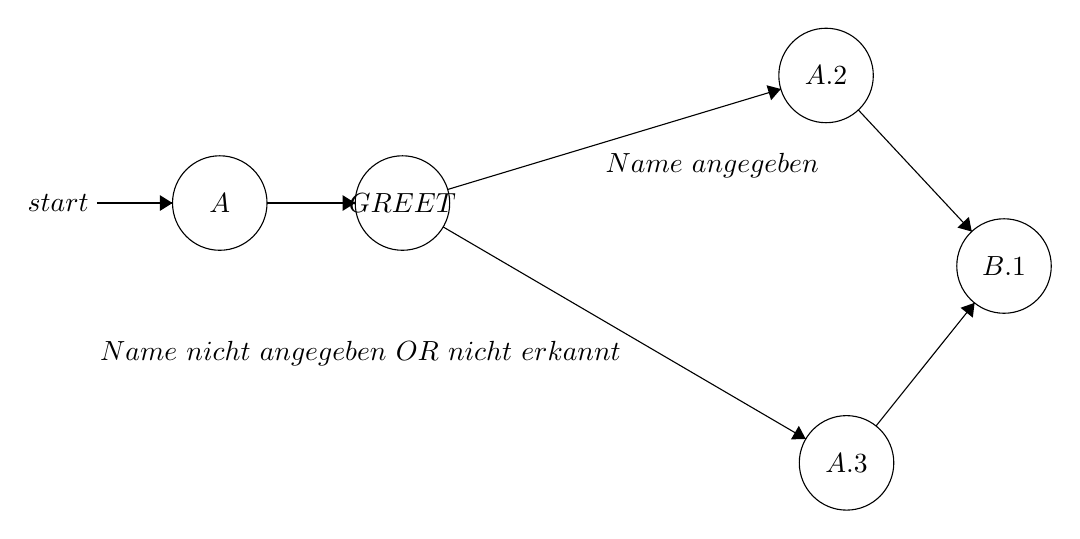
\begin{tikzpicture}[scale=0.2]
\tikzstyle{every node}+=[inner sep=0pt]
\draw [black] (11.5,-26.9) circle (3);
\draw (11.5,-26.9) node {$A$};
\draw [black] (50,-18.8) circle (3);
\draw (50,-18.8) node {$A.2$};
\draw [black] (51.3,-43.4) circle (3);
\draw (51.3,-43.4) node {$A.3$};
\draw [black] (23.1,-26.9) circle (3);
\draw (23.1,-26.9) node {$GREET$};
\draw [black] (61.3,-30.9) circle (3);
\draw (61.3,-30.9) node {$B.1$};
\draw [black] (3.7,-26.9) -- (8.5,-26.9);
\draw (3.2,-26.9) node [left] {$start$};
\fill [black] (8.5,-26.9) -- (7.7,-26.4) -- (7.7,-27.4);
\draw [black] (14.5,-26.9) -- (20.1,-26.9);
\fill [black] (20.1,-26.9) -- (19.3,-26.4) -- (19.3,-27.4);
\draw [black] (25.97,-26.04) -- (47.13,-19.66);
\fill [black] (47.13,-19.66) -- (46.22,-19.42) -- (46.51,-20.37);
\draw (42.77,-23.71) node [below] {$Name\mbox{ }angegeben$};
\draw [black] (25.69,-28.42) -- (48.71,-41.88);
\fill [black] (48.71,-41.88) -- (48.27,-41.05) -- (47.77,-41.91);
\draw (20.43,-35.67) node [below] {$Name\mbox{ }nicht\mbox{ }angegeben\mbox{ }OR\mbox{ }nicht\mbox{ }erkannt$};
\draw [black] (53.17,-41.06) -- (59.43,-33.24);
\fill [black] (59.43,-33.24) -- (58.54,-33.55) -- (59.32,-34.18);
\draw [black] (52.05,-20.99) -- (59.25,-28.71);
\fill [black] (59.25,-28.71) -- (59.07,-27.78) -- (58.34,-28.46);
\end{tikzpicture}
\end{center}


\section{Kaufabsicht}
\label{sec:Kaufabsicht}

Folgendes gilt:

\begin{enumerate}
\item{B.1 ist STARTKAUF}
\item{B.2 ist die Nachfrage, ob ein Kaufwunsch besteht}
\item{B.3 ist die Regel nach Angabe, dass man ein Geschenk bzw. etwas zu einer Anwendung möchte}
\item{X.A ist \texttildelow ende.ASKIFHAPPY}
\item{C.1 ist keyexprodukteigenschaften.STARTPRODUKTEIGENSCHAFTEN bzw. keyexonesentence.STARTKAUF}
\item{Die restlichen Zustände sind nach ihren Regeln benannt}
\end{enumerate}

Von der Regel STARTKAUF geht der Bot in INTRO über und fragt, ob ein Kaufwunsch besteht. Dies wird so lange erfragt, bis der Bot die Antwort des Nutzers verstanden hat.\\
Besteht kein Kaufwunsch, erfolgt erneute Nachfrage. Bestätigt der Nutzer, dass er nichts kaufen möchte, so wird dieser zu Regel ASKIFHAPPY im Topic Ende weitergeleitet. Besteht doch ein Kaufwunsch, so wird er in die Regel FIRSTQ weitergeleitet. Sollten Probleme mit der Initialisierung der Datenbank auftreten, so wird dieser Zustand so lange wiederholt, bis die Datenbank aktiviert werden kann. \\
In FIRSTQ wird der Nutzer gefragt, ob dieser etwas zum Verschenken oder anhand eines Anwendungszweck sucht. Nennt der Nutzer nur, dass er ein Geschenk beziehungsweise etwas für einen gegebenen Zweck sucht, so wird ihm vorgeschlagen, welche Geschenkideen beziehungsweise Anwendungszwecke zur Verfügung stehen. Der Nutzer muss eine der aufgelisteten Geschenkideen oder Anwendungszwecke bennen, welche als Variable abgespeichert werden. Nennt der Nutzer stattdessen direkt, was für eine Geschenkidee oder Anwendungszweck er möchte und ist dies auch bekannt, dann muss die Absicht nicht weiter konkretisiert werden und wird in einer Variable abgespeichert. \\
Danach betritt der Bot die Regel keyexprodukteigenschaften.STARTPRODUKTEIGENSCHAFTEN bzw. keyexonesentence.STARTKAUF, abhängig vom vorliegenden Ansatz (beide Ansätze im Projekt enthalten, s. \ref{sec:Versionen}). 

\begin{center}
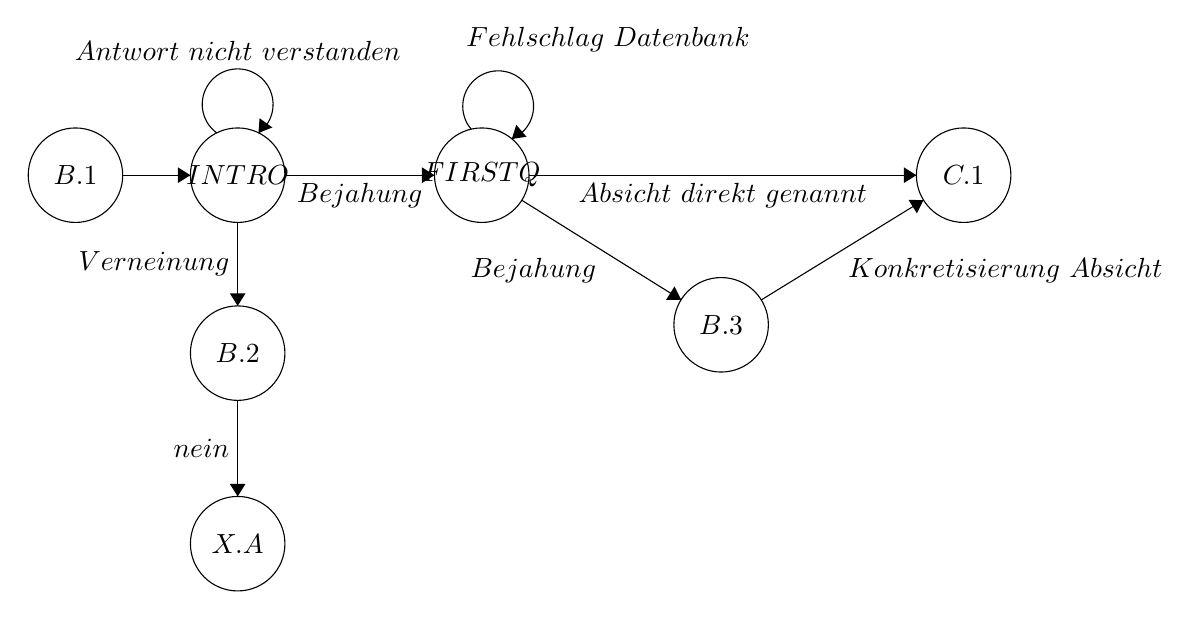
\begin{tikzpicture}[scale=0.2]
\tikzstyle{every node}+=[inner sep=0pt]
\draw [black] (4.7,-30) circle (3);
\draw (4.7,-30) node {$B.1$};
\draw [black] (15,-30) circle (3);
\draw (15,-30) node {$INTRO$};
\draw [black] (15,-41.3) circle (3);
\draw (15,-41.3) node {$B.2$};
\draw [black] (15,-53.4) circle (3);
\draw (15,-53.4) node {$X.A$};
\draw [black] (30.5,-30) circle (3);
\draw (30.5,-30) node {$FIRSTQ$};
\draw [black] (45.7,-39.5) circle (3);
\draw (45.7,-39.5) node {$B.3$};
\draw [black] (61.1,-30) circle (3);
\draw (61.1,-30) node {$C.1$};
\draw [black] (7.7,-30) -- (12,-30);
\fill [black] (12,-30) -- (11.2,-29.5) -- (11.2,-30.5);
\draw [black] (15,-33) -- (15,-38.3);
\fill [black] (15,-38.3) -- (15.5,-37.5) -- (14.5,-37.5);
\draw (14.5,-35.65) node [left] {$Verneinung$};
\draw [black] (15,-44.3) -- (15,-50.4);
\fill [black] (15,-50.4) -- (15.5,-49.6) -- (14.5,-49.6);
\draw (14.5,-47.35) node [left] {$nein$};
\draw [black] (18,-30) -- (27.5,-30);
\fill [black] (27.5,-30) -- (26.7,-29.5) -- (26.7,-30.5);
\draw (22.75,-30.5) node [below] {$Bejahung$};
\draw [black] (13.677,-27.32) arc (234:-54:2.25);
\draw (15,-22.75) node [above] {$Antwort\mbox{ }nicht\mbox{ }verstanden$};
\fill [black] (16.32,-27.32) -- (17.2,-26.97) -- (16.39,-26.38);
\draw [black] (33.5,-30) -- (58.1,-30);
\fill [black] (58.1,-30) -- (57.3,-29.5) -- (57.3,-30.5);
\draw (45.8,-30.5) node [below] {$Absicht\mbox{ }direkt\mbox{ }genannt$};
\draw [black] (48.25,-37.92) -- (58.55,-31.58);
\fill [black] (58.55,-31.58) -- (57.6,-31.57) -- (58.13,-32.42);
\draw (63.75,-35.26) node [below] {$Konkretisierung\mbox{ }Absicht$};
\draw [black] (33.04,-31.59) -- (43.16,-37.91);
\fill [black] (43.16,-37.91) -- (42.74,-37.06) -- (42.21,-37.91);
\draw (33.77,-35.25) node [below] {$Bejahung$};
\draw [black] (29.834,-27.087) arc (220.60377:-67.39623:2.25);
\draw (38.52,-22.23) node [above] {$Fehlschlag\mbox{ }Datenbank$};
\fill [black] (32.41,-27.7) -- (33.34,-27.56) -- (32.69,-26.8);
\end{tikzpicture}
\end{center}


\section{KeyExProdukteigenschaften}
\label{sec:KeyExProdukteigenschaften}

Folgendes gilt:

\begin{enumerate}
\item{C.1 ist STARTPRODUKTEIGENSCHAFTEN}
\item{C.2a ist ASKNAME}
\item{C.2b ist KIND}
\item{C.3 ist DESIGN}
\item{C.4 ist PRICE }
\item{C.5 ist SUMMARY }
\item{D.1 ist \texttildelow dbsearch.WELCOME}
\end{enumerate}


Wird die Version Produkteigeschaften gewählt, so erfolgt ein einzelnes Erfragen der jeweiligen Eigenschaften.\\
In der Regel gilt: Werden in den Eingaben Stichworte erkannt, die als Eigenschaften in der Datenbank bekannt sind, so werden diese in Variablen gespeichert (s. \ref{sec:ChatScript: Pattern-Matching}).\\
Zunächst wird gefragt, ob der Nutzer sein gewünschtes Produkt beim Produktnamen kennt. Ist dies nicht der Fall oder wird die Eingabe nicht als Name identifiziert, wird gefragt, ob der Nutzer weiß, von welcher Kategorie, zum Beispiel Kleidung oder Buch seine Idee ist. Erfolgt eine Eingabe, die im Konzept \texttildelow art bekannt ist, so wird in der entsprechenden Variable \lstinline|$art| dieser Wert gespeichert.\\
Daraufhin wird gefragt, ob der Kunde etwas zur Ausführung, zum Beispiel Farbe oder Sprache, sagen kann. Wird eine bekannte Ausführung erkannt, so wird diese gespeichert, ansonsten wird die Eingabe ignoriert.\\
Im Anschluss wird erfragt, welchen Preis man maximal zahlen möchte. Hierbei muss als Preislimit eine positive Integerzahl angegeben werden.\\ 
In SUMMARY wird zusammengefasst, was der Bot erkennen konnte und fragt den Nutzer, ob dies seinem Wunsch entspricht. Ist dies der Fall, so betritt der Bot die Regel WELCOME in Dbsearch, ansonsten wird bei STARTPRODUKTEIGENSCHAFTEN von Vorne angefangen. Für die Zusammenfassung wurden ab FIRSTQ ein entsprechender Satz in der Variable \lstinline|$zusammenfassung| gespeichert, sodass in SUMMARY ein zusammenhängender Text ausgegeben werden kann.



\begin{center}
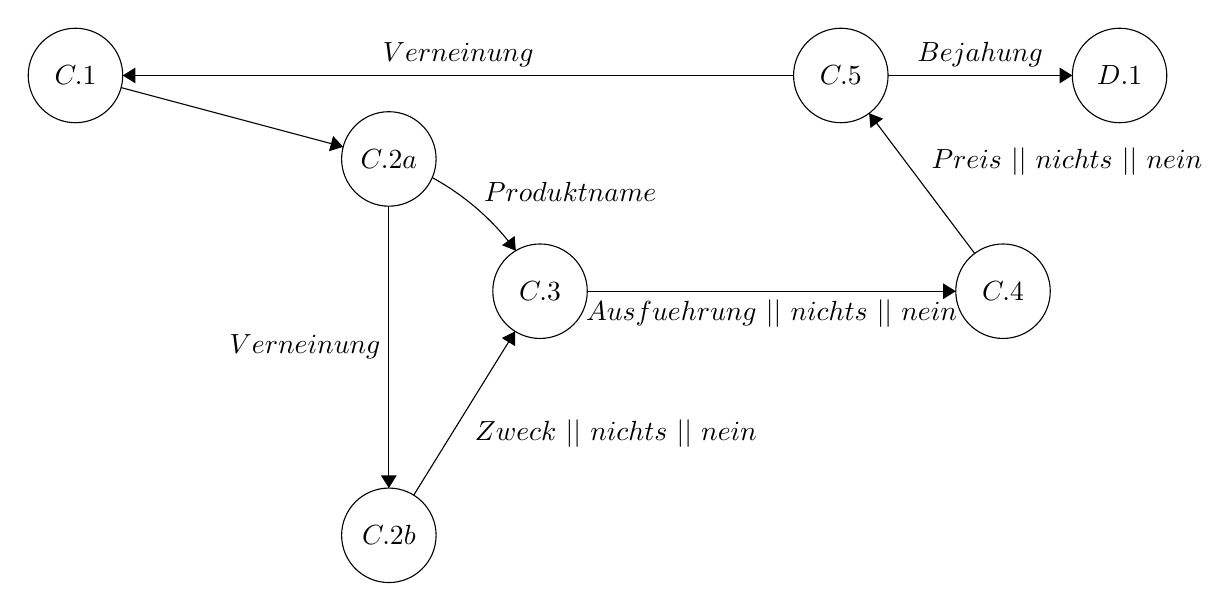
\begin{tikzpicture}[scale=0.2]
\tikzstyle{every node}+=[inner sep=0pt]
\draw [black] (8.2,-16.1) circle (3);
\draw (8.2,-16.1) node {$C.1$};
\draw [black] (28.1,-21.4) circle (3);
\draw (28.1,-21.4) node {$C.2a$};
\draw [black] (28.1,-45.3) circle (3);
\draw (28.1,-45.3) node {$C.2b$};
\draw [black] (37.7,-29.8) circle (3);
\draw (37.7,-29.8) node {$C.3$};
\draw [black] (67.1,-29.8) circle (3);
\draw (67.1,-29.8) node {$C.4$};
\draw [black] (56.8,-16.1) circle (3);
\draw (56.8,-16.1) node {$C.5$};
\draw [black] (74.5,-16.1) circle (3);
\draw (74.5,-16.1) node {$D.1$};
\draw [black] (11.1,-16.87) -- (25.2,-20.63);
\fill [black] (25.2,-20.63) -- (24.56,-19.94) -- (24.3,-20.91);
\draw [black] (30.852,-22.584) arc (61.41227:36.21588:16.173);
\fill [black] (36.16,-27.23) -- (36.09,-26.29) -- (35.29,-26.88);
\draw (39.61,-24.12) node [above] {$Produktname$};
\draw [black] (29.68,-42.75) -- (36.12,-32.35);
\fill [black] (36.12,-32.35) -- (35.27,-32.77) -- (36.12,-33.29);
\draw (33.53,-38.84) node [right] {$Zweck\mbox{ }||\mbox{ }nichts\mbox{ }||\mbox{ }nein$};
\draw [black] (40.7,-29.8) -- (64.1,-29.8);
\fill [black] (64.1,-29.8) -- (63.3,-29.3) -- (63.3,-30.3);
\draw (52.4,-30.3) node [below] {$Ausfuehrung\mbox{ }||\mbox{ }nichts\mbox{ }||\mbox{ }nein$};
\draw [black] (65.3,-27.4) -- (58.6,-18.5);
\fill [black] (58.6,-18.5) -- (58.68,-19.44) -- (59.48,-18.84);
\draw (62.53,-21.55) node [right] {$Preis\mbox{ }||\mbox{ }nichts\mbox{ }||\mbox{ }nein$};
\draw [black] (28.1,-24.4) -- (28.1,-42.3);
\fill [black] (28.1,-42.3) -- (28.6,-41.5) -- (27.6,-41.5);
\draw (27.6,-33.35) node [left] {$Verneinung$};
\draw [black] (53.8,-16.1) -- (11.2,-16.1);
\fill [black] (11.2,-16.1) -- (12,-16.6) -- (12,-15.6);
\draw (32.5,-15.6) node [above] {$Verneinung$};
\draw [black] (59.8,-16.1) -- (71.5,-16.1);
\fill [black] (71.5,-16.1) -- (70.7,-15.6) -- (70.7,-16.6);
\draw (65.65,-15.6) node [above] {$Bejahung$};
\end{tikzpicture}
\end{center}


\section{KeyExOnesentence}
\label{sec:KeyExOnesentence}

Folgendes gilt: 

\begin{enumerate}
\item{C.1 ist STARTONESENTENCE}
\item{C.X ist QUALITY}
\item{C.5 ist SUMMARY}
\item{D.1 ist \texttildelow dbsearch.WELCOME}
\end{enumerate}

In KeyExOnesentence kommt der in Abschnitt \ref{sec:ChatScript: Pattern-Matching} zum Pattern-Matching besprochene Ansatz zur Extrahierung mehrerer Informationen aus einem einzelnen Satz zum Tragen.\\
In QUALITY anhand der Nutzereingabe ermittelt, um welches der insgesamt 11 Muster es sich dabei der Nutzereingabe handelt und die Informationen entsprechend extrahiert. Es gibt 9 Muster zur Eingabe der Produkteingenschaften und 2 Muster für den Fall, dass der Kunde keine Angaben machen kann.\\
In SUMMARY wird zusammengefasst, was der Bot erkennen konnte und fragt den Nutzer, ob dies seinem entspricht. Ist dies der Fall, so betritt der Bot die Regel WELCOME in Dbsearch, ansonsten wird bei STARTPONESENTENCE von Vorne angefangen. Für die Zusammenfassung wurden ab FIRSTQ ein entsprechender Satz in der Variable \lstinline|$zusammenfassung| gespeichert, sodass in SUMMARY ein zusammenhängender Text ausgegeben werden kann.

\begin{center}
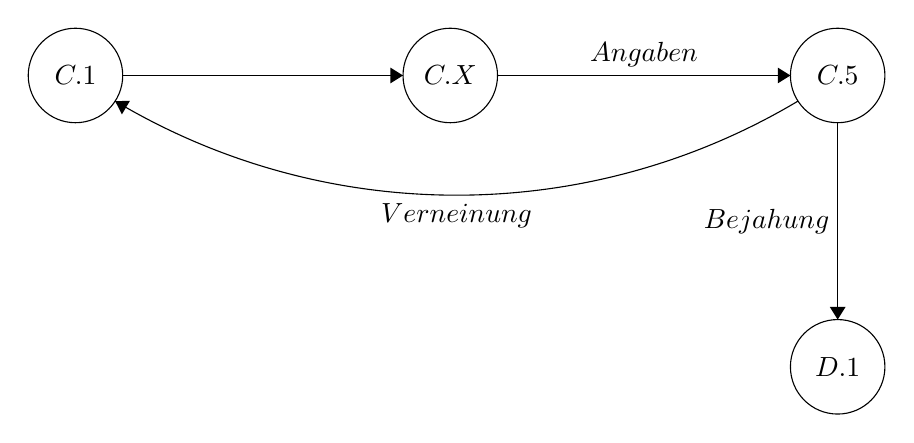
\begin{tikzpicture}[scale=0.2]
\tikzstyle{every node}+=[inner sep=0pt]
\draw [black] (5.4,-30.8) circle (3);
\draw (5.4,-30.8) node {$C.1$};
\draw [black] (29.2,-30.8) circle (3);
\draw (29.2,-30.8) node {$C.X$};
\draw [black] (53.8,-30.8) circle (3);
\draw (53.8,-30.8) node {$C.5$};
\draw [black] (53.8,-49.3) circle (3);
\draw (53.8,-49.3) node {$D.1$};
\draw [black] (8.4,-30.8) -- (26.2,-30.8);
\fill [black] (26.2,-30.8) -- (25.4,-30.3) -- (25.4,-31.3);
\draw [black] (32.2,-30.8) -- (50.8,-30.8);
\fill [black] (50.8,-30.8) -- (50,-30.3) -- (50,-31.3);
\draw (41.5,-30.3) node [above] {$Angaben$};
\draw [black] (53.8,-33.8) -- (53.8,-46.3);
\fill [black] (53.8,-46.3) -- (54.3,-45.5) -- (53.3,-45.5);
\draw (53.3,-40.05) node [left] {$Bejahung$};
\draw [black] (51.28,-32.427) arc (-59.18008:-120.81992:42.316);
\fill [black] (7.92,-32.43) -- (8.35,-33.27) -- (8.86,-32.41);
\draw (29.6,-38.9) node [below] {$Verneinung$};
\end{tikzpicture}
\end{center}


\section{Dbsearch}
\label{sec:Dbsearch}

Folgendes gilt: 

\begin{enumerate}
\item{D.1 ist WELCOME}
\item{D.2 ist SEARCHCREATE}
\item{D.3 ist SEARCHPRODUCT}
\item{D.4 ist PRODUCTNAME}
\item{D.5 ist PRODUCTDESCR}
\item{D.6 ist PRODUCTPRICE}
\item{D.7 ist RESPONSE}
\item{D.X ist SEARCHAGAIN}
\item{X.S ist \texttildelow ende.SETNULLREP}
\item{X.A ist \texttildelow ende.ASKIFHAPPY}
\end{enumerate}

Basierend auf den ermittelten Nutzerinformationen wird nun eine Query erstellt. Dabei wird für jeden Nutzer in der Regel SEARCHCREATE eine eigene Tabelle erstellt, die eine Kopie der originalen Datenbank ist.\\
Daraufhin wird der Schritt SEARCHPRODUCT betreten, in der nach Artikeln, die der Beschreibung des Nutzers entsprechen, gesucht wird. In den den folgenden drei Regeln PRODUCTNAME, PRODUCTDESCR und PRODUCTPRICE wird der Name, die Beschreibung beziehungsweise der Preis eines der gefundenen Produkte aus der Datenbank vorgestellt.\\
In ReESPONSE wird gefragt, ob das Produkt dem Nutzerwunsch entspricht. Ist dies nicht der Fall, so wird in SEARCHAGAIN übergegangen und erneut gesucht, wobei das bereits gefundene Produkt aufgrund Eigenschaft queried in der Datenbank (s. \ref{sec:queried}) nicht erneut gefunden werden kann. Ist der Nutzer hingegen zufrieden, so wird dieser gefragt, ob er noch ein Produkt suchen, bereits ausgewählte Artikel einsehen möchte oder ob er fertig ist.\\
Ist Ersteres der Fall, so wird in die Regel SETNULLANDREP im Topic Ende weitergeleitet, sodass eine erneute Suche möglich ist. Ist Zweiteres der Fall, so wird in der Datenbank erneut anhand der queried-Eigenschaft eine Anfrage für alle Produkte aufgerufen, die akzeptiert worden sind. Will der Nutzer kein weiteres Produkt mehr suchen, so wird die Regel ASKIFHAPPY in Ende betreten.  
\begin{center}
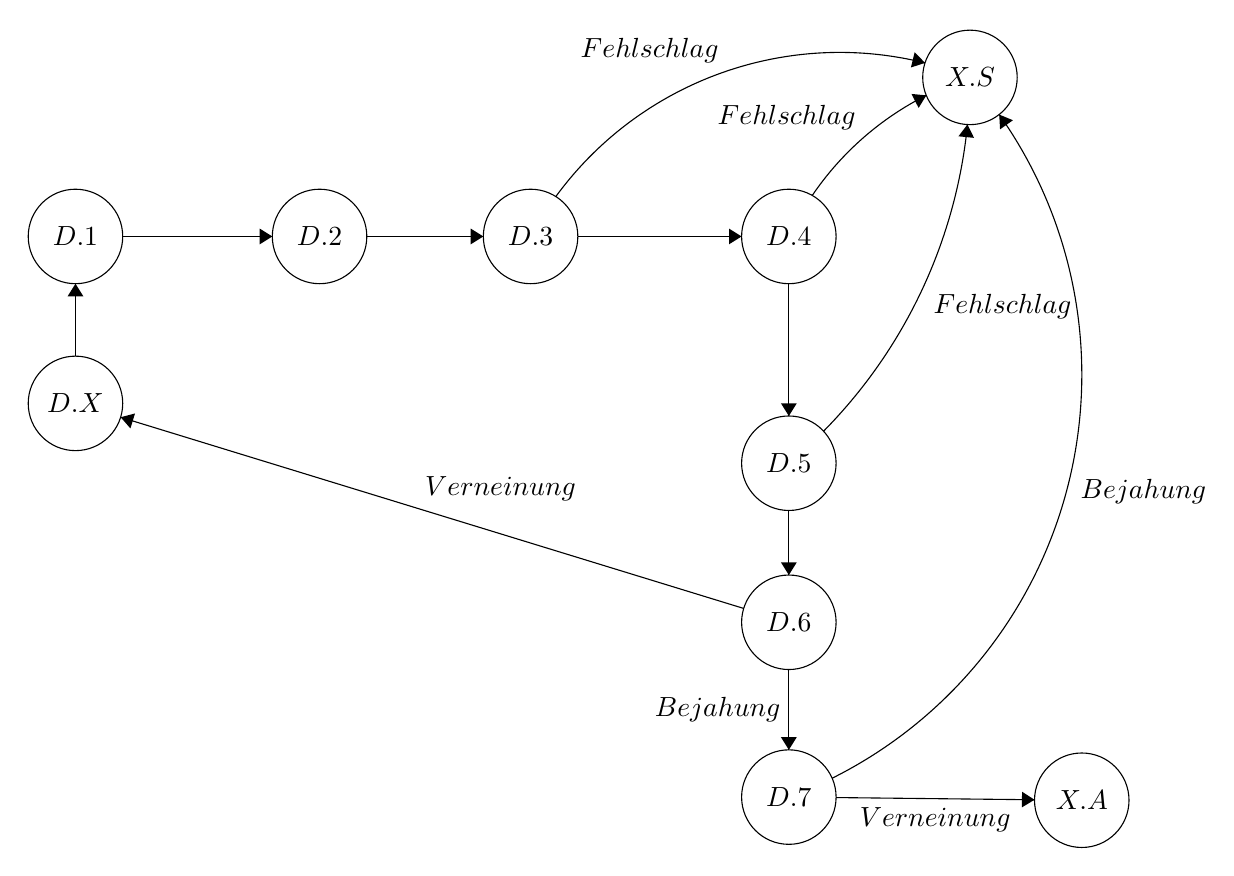
\begin{tikzpicture}[scale=0.2]
\tikzstyle{every node}+=[inner sep=0pt]
\draw [black] (8.1,-14.5) circle (3);
\draw (8.1,-14.5) node {$D.1$};
\draw [black] (23.6,-14.5) circle (3);
\draw (23.6,-14.5) node {$D.2$};
\draw [black] (37,-14.5) circle (3);
\draw (37,-14.5) node {$D.3$};
\draw [black] (64.9,-4.4) circle (3);
\draw (64.9,-4.4) node {$X.S$};
\draw [black] (53.4,-14.5) circle (3);
\draw (53.4,-14.5) node {$D.4$};
\draw [black] (53.4,-28.9) circle (3);
\draw (53.4,-28.9) node {$D.5$};
\draw [black] (8.1,-25.1) circle (3);
\draw (8.1,-25.1) node {$D.X$};
\draw [black] (53.4,-39) circle (3);
\draw (53.4,-39) node {$D.6$};
\draw [black] (53.4,-50.1) circle (3);
\draw (53.4,-50.1) node {$D.7$};
\draw [black] (72,-50.3) circle (3);
\draw (72,-50.3) node {$X.A$};
\draw [black] (11.1,-14.5) -- (20.6,-14.5);
\fill [black] (20.6,-14.5) -- (19.8,-14) -- (19.8,-15);
\draw [black] (26.6,-14.5) -- (34,-14.5);
\fill [black] (34,-14.5) -- (33.2,-14) -- (33.2,-15);
\draw [black] (38.603,-11.967) arc (143.8353:75.96593:22.332);
\fill [black] (62.05,-3.48) -- (61.39,-2.8) -- (61.15,-3.77);
\draw (44.56,-3.51) node [above] {$Fehlschlag$};
\draw [black] (54.885,-11.897) arc (145.81813:116.76502:19.213);
\fill [black] (62.13,-5.54) -- (61.19,-5.45) -- (61.64,-6.34);
\draw (53.26,-7.77) node [above] {$Fehlschlag$};
\draw [black] (53.4,-17.5) -- (53.4,-25.9);
\fill [black] (53.4,-25.9) -- (53.9,-25.1) -- (52.9,-25.1);
\draw [black] (40,-14.5) -- (50.4,-14.5);
\fill [black] (50.4,-14.5) -- (49.6,-14) -- (49.6,-15);
\draw [black] (64.743,-7.395) arc (-5.65741:-44.63217:32.239);
\fill [black] (64.74,-7.39) -- (64.17,-8.14) -- (65.16,-8.24);
\draw (62.56,-18.96) node [right] {$Fehlschlag$};
\draw [black] (8.1,-22.1) -- (8.1,-17.5);
\fill [black] (8.1,-17.5) -- (7.6,-18.3) -- (8.6,-18.3);
\draw [black] (53.4,-31.9) -- (53.4,-36);
\fill [black] (53.4,-36) -- (53.9,-35.2) -- (52.9,-35.2);
\draw [black] (53.4,-42) -- (53.4,-47.1);
\fill [black] (53.4,-47.1) -- (53.9,-46.3) -- (52.9,-46.3);
\draw (52.9,-44.55) node [left] {$Bejahung$};
\draw [black] (50.53,-38.12) -- (10.97,-25.98);
\fill [black] (10.97,-25.98) -- (11.59,-26.69) -- (11.88,-25.74);
\draw (35.09,-31.31) node [above] {$Verneinung$};
\draw [black] (66.756,-6.755) arc (35.24029:-63.48971:28.636);
\fill [black] (66.76,-6.76) -- (66.81,-7.7) -- (67.63,-7.12);
\draw (71.9,-30.73) node [right] {$Bejahung$};
\draw [black] (56.4,-50.13) -- (69,-50.27);
\fill [black] (69,-50.27) -- (68.21,-49.76) -- (68.19,-50.76);
\draw (62.69,-50.75) node [below] {$Verneinung$};
\end{tikzpicture}
\end{center}


\section{Ende}
\label{sec:Ende}

Folgendes gilt:

\begin{enumerate}
\item{X.A ist ASKIFHAPPY}
\item{X.B ist STILLHELP}
\item{X.C ist das Ablehnen einer weiteren Suche}
\item{\textcolor[rgb]{1,0.41,0.13}{X.D ist fgt}} %% IST DAS FORGET? FORGET kann raus.
\item{X.E ist GOODBYE}
\item{X.S ist SETNULLREP}
\item{FIRSTQ ist FIRSTQ aus Kaufabsicht}
\item{Z ist ein anderer Endzustand}
\end{enumerate}

Wird die Regel ASKIFHAPPY in Ende betreten, so wird dem Nutzer die Frage gestellt, ob der Bot noch was für ihn tun könne oder nicht.\\
Ist dies nicht der Fall, so wird im Folgenden die eigene Tabelle des Nutzers gelöscht und der Bot beendet (X.E). Ist dies jedoch der Fall, so wird in STILLHELP gefragt, ob man eine neue Suche starten möchte. Wenn nicht, so wird der Bot beendet. Andererseits wird in SETNULLUNDREP übergegangen, wo die für die Kaufberatung relevanten Variablen zurückgesetzt werden und anschließend FIRSTQ im Topic Kaufabsicht zur erneuten Suche eines Produkts betreten. 

\begin{center}
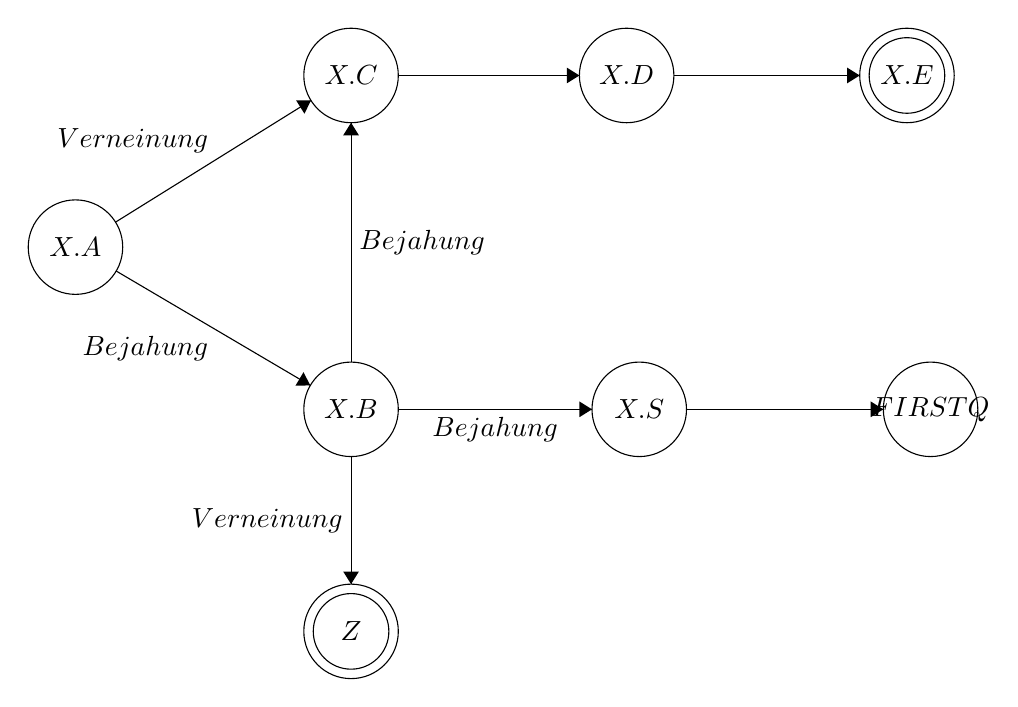
\begin{tikzpicture}[scale=0.2]
\tikzstyle{every node}+=[inner sep=0pt]
\draw [black] (6.7,-28.2) circle (3);
\draw (6.7,-28.2) node {$X.A$};
\draw [black] (24.2,-38.5) circle (3);
\draw (24.2,-38.5) node {$X.B$};
\draw [black] (24.2,-17.3) circle (3);
\draw (24.2,-17.3) node {$X.C$};
\draw [black] (24.2,-52.6) circle (3);
\draw (24.2,-52.6) node {$Z$};
\draw [black] (24.2,-52.6) circle (2.4);
\draw [black] (41.7,-17.3) circle (3);
\draw (41.7,-17.3) node {$X.D$};				%% FORGET kann raus!! Ist das FORGET?
\draw [black] (59.5,-17.3) circle (3);
\draw (59.5,-17.3) node {$X.E$};
\draw [black] (59.5,-17.3) circle (2.4);
\draw [black] (42.5,-38.5) circle (3);
\draw (42.5,-38.5) node {$X.S$};
\draw [black] (61,-38.5) circle (3);
\draw (61,-38.5) node {$FIRSTQ$};
\draw [black] (9.29,-29.72) -- (21.61,-36.98);
\fill [black] (21.61,-36.98) -- (21.18,-36.14) -- (20.67,-37);
\draw (11.13,-33.85) node [below] {$Bejahung$};
\draw [black] (9.25,-26.61) -- (21.65,-18.89);
\fill [black] (21.65,-18.89) -- (20.71,-18.88) -- (21.24,-19.73);
\draw (10.34,-22.25) node [above] {$Verneinung$};
\draw [black] (24.2,-35.5) -- (24.2,-20.3);
\fill [black] (24.2,-20.3) -- (23.7,-21.1) -- (24.7,-21.1);
\draw (24.7,-27.9) node [right] {$Bejahung$};
\draw [black] (24.2,-41.5) -- (24.2,-49.6);
\fill [black] (24.2,-49.6) -- (24.7,-48.8) -- (23.7,-48.8);
\draw (23.7,-45.55) node [left] {$Verneinung$};
\draw [black] (27.2,-17.3) -- (38.7,-17.3);
\fill [black] (38.7,-17.3) -- (37.9,-16.8) -- (37.9,-17.8);
\draw [black] (44.7,-17.3) -- (56.5,-17.3);
\fill [black] (56.5,-17.3) -- (55.7,-16.8) -- (55.7,-17.8);
\draw [black] (27.2,-38.5) -- (39.5,-38.5);
\fill [black] (39.5,-38.5) -- (38.7,-38) -- (38.7,-39);
\draw (33.35,-39) node [below] {$Bejahung$};
\draw [black] (45.5,-38.5) -- (58,-38.5);
\fill [black] (58,-38.5) -- (57.2,-38) -- (57.2,-39);
\end{tikzpicture}
\end{center}
